\section{The Prismatic High-Temperature Gas-Cooled Reactor}
\label{sec:pmr}

% History
The history of prismatic \glspl{HTGR} or simply \glspl{PMR} began in the 1960s with the deployment of the Dragon reactor in the \gls{UK} \cite{brey_development_2001}.
Its initial objective was to demonstrate the feasibility of \glspl{HTGR}.
The Dragon reactor experiment first operated in July 1965 and reached its full-power operation of 20 MWth in April 1966.
The reactor operated for 11 years, demonstrating many components' successful operation and providing information on fuel and material irradiation.
Simultaneously, interest in the \gls{US} led to the 40 MWe \gls{HTGR} Peach Bottom Unit 1.
This reactor achieved initial criticality in March 1966 and went into commercial operation in June 1967.
Peach Bottom demonstrated the \gls{HTGR} concept by confirming the core physics calculations, verifying the design analysis methods, and providing a database for further design activities.
Most importantly, the plant demonstrated that \glspl{HTGR} can load follow \cite{brey_development_2001}.
After the deployment of these two prototype reactors came the first \gls{HTGR} large-scale demonstration plant - the Fort St. Vrain Generating Station.
Its electric power generation started in December 1976, reaching full-power operation in November 1981.
The Fort St. Vrain plant generated 842 MWt to achieve a net output of 330 MWe.
This reactor laid the foundation for future prismatic designs.
Beginning with Fort St. Vrain, the prismatic HTGRs in the \gls{US} adopted as their fuel large hexagonal-shaped graphite elements with ceramic coated \gls{TRISO} particles embedded within rods  \cite{brey_development_2001}.
% Despite these plants did not demonstrate the commercial capabilities of the \glspl{PMR}, they were  valuable in demonstrating attributes as the performance of the \gls{TRISO} fuel particles \cite{herranz_power_2009}.

% Safety characteristics of HTGRs: TRISO fuel
The HTGR's most fundamental characteristic is its unique safety features.
Radionuclide containment does not rely on active systems or operator actions.
\gls{TRISO} particles, pictured in Figure \ref{fig:triso}, play a significant role in this task.
They consist of various layers acting as containment to limit radioactive product release.
A \gls{TRISO} particle is a microsphere of about 0.8 mm in diameter.
It includes a fuel kernel surrounded by a porous carbon layer (or buffer), followed successively by an \gls{IPyC} layer, a \gls{SiC} layer, and an \gls{OPyC} layer.
The buffer layer limits kernel migration and provides some retention of gas compounds \cite{oecd_nea_benchmark_2017}.
The \gls{IPyC} layer protects the kernel from chloride in the event of \gls{SiC} decomposition and contributes to fission gas retention \cite{demkowickz_paul_triso_2019}.
The \gls{SiC} layer ensures the particle's structural integrity under constant pressure and helps retain non-gaseous fission products.
The \gls{OPyC} layer contributes to fission gas retention and protects the \gls{SiC} layer during handling.
As an additional advantage, \gls{TRISO} particles increase the proliferation resistance of \glspl{HTGR}.
TRISO particles provide significant barriers and technical difficulties to retrieve materials from within the fuel coatings \cite{paviet-hartmann_analysis_2011}.
The particles can sustain high burnup, which causes the used nuclear fuel to have a low volume fraction of plutonium.
Such a low fraction of plutonium makes the fuel unsuitable for use in weapons \cite{paviet-hartmann_analysis_2011}.

\begin{figure}[htbp!]
	\centering
	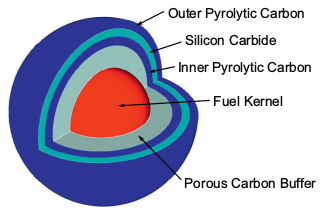
\includegraphics[height=3.5cm]{figures/triso}
	\caption{Drawing of a TRISO fuel particle. Image reproduced from \cite{hales_multidimensional_2013}.}
	\label{fig:triso}
\end{figure}

% Safety characteristics of HTGRs: Graphite and negative temp coeff
Graphite is another contributor to the passive safety of the \gls{HTGR} design.
Combining ceramic fuel and a graphite core structure permits high operating temperatures \cite{ballinger_balance_2004}.
Graphite has a high heat capacity and maintains its strength at temperatures beyond 2760 $^{\circ}$C.
Additionally, HTGRs have a negative temperature coefficient of reactivity and a low core power density.
A low core power density enables passive heat transfer mechanisms to remove the decay heat following postulated accidents \cite{neylan_modular_1988}.
These passive heat transfer mechanisms rely primarily on the natural processes of conduction, thermal radiation, and convection.
As a result, temperature changes in the core occur slowly and without damage to the core structure during transients.

% Co-generation applications: Rankine vs Bryton
HTGRs higher operating temperatures are a desirable feature because they offer increased thermal conversion efficiencies.
The early \gls{HTGR} designs converted their heat into electricity using the steam-Rankine cycle \cite{herranz_power_2009}.
In such a system, the helium coolant passes through a steam generator, and the steam drives a turbine.
This arrangement is around 38\% efficient \cite{breeze_nuclear_2014}.
However, the steam cycle requires a steam generator and also a gas circulator \cite{no_review_2007}.
This requirement increases the capital cost of power plant, and it creates a risk of a water ingress event.
The Brayton cycle is a better option because the helium coolant can directly drive a gas turbine in a closed cycle.
A closed cycle eliminates the need for a steam generator and a gas circulator.
Additionally, it removes external sources of contamination of the nuclear circuit, reducing the need for on-line cleanup systems \cite{iaea_current_2001}.
With the Brayton cycle, the system can achieve an energy conversion efficiency of around 48\% \cite{breeze_nuclear_2014}.

Higher outlet temperatures and increased thermal conversion efficiencies in HTGRs enable a wide range of process heat applications, such as coal gasification processes, oil refinery processes, and production of synthesis gas, methanol, and hydrogen.
Hydrogen offers a solution to energy and climate challenges, decarbonizing the transport and power sectors \cite{nagashima_japans_2018}.
Several hydrogen production processes benefit from high temperatures, such as high-temperature electrolysis \cite{doenitz_hydrogen_1980} or thermochemical water-splitting \cite{yildiz_efficiency_2006}.
Utilizing the \gls{HTGR} as the process energy source eliminates the need to burn fossil fuels to generate the steam those processes require \cite{iaea_current_2001}.

% Maybe this paragraph should be in objectives
This thesis focuses primarily on the \gls{MHTGR}-350 \cite{neylan_modular_1988} \cite{silady_licensing_1988}.
Under the sponsorship of the \gls{US} \gls{DOE}, a team consisting of General Atomics, Combustion Engineering, General Electric, Bechtel National, Stone \& Webster Engineering, and \gls{ORNL} developed the \gls{MHTGR}-350 \cite{neylan_modular_1988}.
They designed the basic module to deliver superheated steam at 17.3 MPa and 538 $^{\circ}$C.
Based on both economic and technological considerations, a 350 MWth modular reactor defines the optimal configuration.
The team completed in 1986 the preliminary safety information document for the MHTGR-350 and the complete draft pre-application in 1989 \cite{huning_steady_2014}.

% \cite{ballinger_balance_2004}
% The modular type HTGR provides the extra unique characteristic that the fuel temperature will not exceed the failure temperature following postulated accidents just by using passive heat transfer mechanisms.

\section{Motivation}

This work's ultimate goal is to support the development of \gls{HTGR} technology.
More specifically, we focus on the development of computational methods for modeling \glspl{HTGR} with \textit{Moltres} \cite{lindsay_introduction_2018} as our primary analysis tool.

% Why do we focus on HTGRs?
The Generation IV Roadmap project identified reactor concepts that could meet the future's energy demands in an efficient, economical, and environmentally safe manner \cite{macdonald_ngnp_2003}.
One of these reactor concepts is the \gls{VHTR}.
A \gls{VHTR} is a type of HTGR whose core outlet temperatures are between 700 and 950 $^{\circ}$C \cite{gif_gif_2019}.
The \gls{DOE} selected this reactor concept for the \gls{NGNP} Project.
This project intended to demonstrate emissions-free nuclear-assisted electricity and hydrogen production by 2015.

Although the \gls{DOE} canceled the \gls{NGNP} Project, the large scale deployment of HTGRs may become a reality in the near term.
Some microreactor designs embody this type of reactor technology and may be operational before 2030.
Additionally, as Section \ref{sec:pmr} has already described, HTGR technology has several favorable characteristics.
To recapitulate the most relevant features, the \gls{HTGR} relies on passive heat transfer mechanisms, uses TRISO particles as its fuel which inhibits proliferation, achieves high temperatures, and benefits from increased cycle efficiencies.
Another beneficial characteristic is that high temperatures enable a wide range of process heat applications, among which we find hydrogen production.

%Why is computational modeling important?
Modeling and prediction of core thermal-hydraulic behavior is necessary for assessing the safety characteristics of a reactor.
Determining the temperature inside a reactor, for both normal and transient operation, is of paramount importance as several materials' integrity depends on it.
Undesirably high temperatures endanger the TRISO particles' integrity and, consequently, jeopardize the fission product containment \cite{tak_numerical_2008}.
% The temperatures in the core have to be kept below values that begin to cause damage to fission product barriers, produce stmctural material weakness, and lead to excessive chemical reaction rates.
Furthermore, the complex fuel blocks geometry requires numerical calculations for obtaining the fuel temperatures.

The characteristics of an \gls{HTGR} are different from those of conventional \glspl{LWR}.
Such differences demand reactor analysis tools that capture the following peculiarities of \glspl{HTGR} \cite{rohde_development_2012}\cite{bostelmann_criticality_2016}:
\begin{itemize}
% \item Hexagonal structure: the shape of the fuel blocks hinders conformity to any orthogonal coordinate system.
\item Double heterogeneity: the TRISO particles form the first heterogeneity level, consisting of four
layers.
The second level arises from the fuel elements, as they encompass the compacts, the coolant, and the moderator.
\item Strong temperature dependence: the fuel temperatures have a significant effect on the neutron spectrum and the transient feedbacks.
\item High temperature gradient: the temperature difference between the fuel and the moderator is large during the course of transients.
\item High thermal inertia: the large graphite structures cause long transients.
\end{itemize}

%Why use Moltres?
Historically, linking a stand-alone neutronics solver to a thermal-hydraulics solver allowed for simulating an entire reactor.
The connection of the programs occurred in a loose-coupling fashion, such that one code's output served as the other's input and vice versa.
This coupling technique is commonly known as the operator-splitting technique \cite{ragusa_consistent_2009}.
In such an approach, each program uses a physical model that solves some of the problem variables while assuming constant the rest of them.
Nonetheless, these physical models describe processes that rely heavily on the solution of one another's.
The neutron flux determines the power distribution, and the power distribution strongly influences the temperature field.
Due to the \gls{HTGR} temperature feedback, the temperature affects the neutron flux distribution in the core.
Because of a strong temperature feedback, multiphysics transient simulations coupled via the operator-splitting approach may introduce significant numerical errors \cite{park_tightly_2010}\cite{ragusa_consistent_2009}.

\gls{MOOSE} \cite{gaston_moose_2009} is a computational framework targeted at solving fully coupled systems.
All the software built on the \gls{MOOSE} framework shares a joint code base.
These features facilitate relatively easy coupling between separate phenomena and allow for great flexibility, even with a large variance in time scales \cite{novak_pronghorn_2018}.
Additionally, all programs use \gls{MPI} for parallel communication and allow for deployment on massively-parallel cluster-computing platforms.

\textit{Moltres} is an open source, \gls{FEM} application built within the \gls{MOOSE} framework.
\textit{Moltres} solves arbitrary-group neutron diffusion, delayed neutron precursor concentration, and temperature governing equations.
All these characteristics, plus some modifications that this work intends to implement, make \textit{Moltres} suitable for solving the type of physical phenomena described above.

\section{Objectives}

% This thesis focuses on steady-state calculations and also intends to set a roadmap for the transient simulations.
As mentioned earlier, the ultimate goal of this work is to support the development of \gls{HTGR} technology.
The following list of main objectives expands on that goal.

\paragraph{Extend Moltres modeling capabilities to \glspl{HTGR}.}
Moltres is a multi-physics solver of \glspl{MSR}.
Enhancing Moltres will allow it to model \glspl{HTGR} as well.

\paragraph{Couple the different physics phenomena present in an HTGR.}
Moltres's current capabilities allow for solving some of the physics in the HTGR design.
Nevertheless, the solver needs to capture the inherent physics in an HTGR and adequately integrate them into the current capabilities.

\paragraph{Develop safety analysis capabilities in Moltres.}
Steady-state simulations help understand the fundamental behavior of an HTGR and, like transient simulations, assist in reactor design. 
Transient simulations also assess the reactor response in design basis events.

\paragraph{Understand \gls{HTGR} contribution to stopping climate change.}
HTGRs are an attractive technology due to attaining high temperatures.
With such high temperatures, the efficiency of hydrogen production increases.

\vskip 0.6cm
The main objectives are somewhat broad.
The following list presents secondary objectives which will lead to the fulfillment of the main objectives:

\paragraph{Predict neutronics.}
Moltres should have the ability to carry out eigenvalue calculations appropriately.
Additionally, Moltres should predict the flux shape and magnitude accurately, during steady-state and transient simulations.

\paragraph{Understand the impact of some simulation parameters.}
The underlying physics of \glspl{HTGR} differ from the physics of other reactors.
Consequently, the simulation results will be sensitive to different parameters from other reactor type simulations.
This work will focus on the energy group structure and its effects on the diffusion calculations.
We will also assess how such parameters affect the performance of the simulations. 

\paragraph{Calculate power distribution correctly.}
The value of an accurate neutronics behavior prediction lies in the accurate prediction of the power distribution.
The power distribution is the most influential parameter over the thermal-hydraulics as it determines the temperature profile in the reactor.

\paragraph{Predict temperature profile accurately.}
Undesirably high temperatures endanger the integrity of the TRISO particles.
Additionally, the temperature influences the neutronics.
Hence, an accurate neutronics calculation will be inaccurate without a correct thermal-hydraulics calculation and vice versa. 

\paragraph{Develop a hydrogen production calculation tool.}
High temperatures enable high-efficiency hydrogen production methods.
Most of them have different energy requirements and production rates.
We will develop a tool to determine such quantities.